\documentclass[pdf]{beamer}
\mode<presentation>{\usetheme{Warsaw}}

%List of packages
\usepackage{graphicx}
\usepackage{caption}
\usepackage{subcaption}
\usepackage[utf8]{inputenc}
\usepackage{amsmath}
\usepackage{tikz}
\usepackage[backend=biber,url=true,doi=true,eprint=false,style=authoryear]{biblatex}

\usetikzlibrary{positioning}
\usetikzlibrary{shapes.geometric}
\usetikzlibrary{fit}
\usetikzlibrary{calc}

\addbibresource{references.bib}

%%%%%%%%%%%
% Metadata
%%%%%%%%%%%

\hypersetup
{
	%Separate multiple authors by comma
  pdfauthor={Renato Lui Geh}
	pdftitle={SPSAS19: Learning Sum-Product networks},
	pdfsubject={Instructions, Tutorials, Guidelines},
	pdfkeywords={SPSAS19, guidelines, presentation format},
	colorlinks=false
}

%%%%%%%%%%%%%%%%
% Title related
%%%%%%%%%%%%%%%%

\setbeamertemplate{subsection in toc}[default]

%The contact for one of the authors MUST be embedded on the title (see below)
\title[Contact: Renato Geh (renatolg@ime.usp.br)]{Learning Sum-Product Networks}
%Subtitle (if needed)
\subtitle{Master's Dissertation}
%For LICENSE, we suggest CC-BY-SA, but you are free to choose your own as long
%as the LICENSE you choose is AT LEAST as permissive as CC-BY-SA
\date[2019]{Institute of Mathematics and Statistics - USP\\\small SPSAS 2019\\ \vspace{0.5cm}
{
\includegraphics[height=0.5cm, keepaspectratio]{8831.png}}\\\vspace{0.30cm} \scriptsize Supported
by CNPq Grant 133787/2019-2}

%If you wish to disable the utf8 inputec package, do not forget
%to use scape characters in your writting if needed, as show below
\author[Renato Geh \hspace{0.2cm} {
\includegraphics[height=0.2cm, keepaspectratio]{8015.png}}]
{\texorpdfstring{Student: Renato Lui Geh\\Advisor: Prof. Dr. Denis Deratani Mauá}{}}

\institute[University of S\~{a}o Paulo (USP)]{University of S\~{a}o Paulo (USP)}


%%%%%%%%%%%%%%%%%%%%%%%%%%%
% Presentation begins here
%%%%%%%%%%%%%%%%%%%%%%%%%%%

\begin{document}

\begin{frame}
	\titlepage
\end{frame}

\section{Motivation}

\begin{frame}
  \frametitle{Motivation}

  What if you could have...\pause

  \begin{figure}
    \begin{subfigure}[b]{.45\textwidth}
      \centering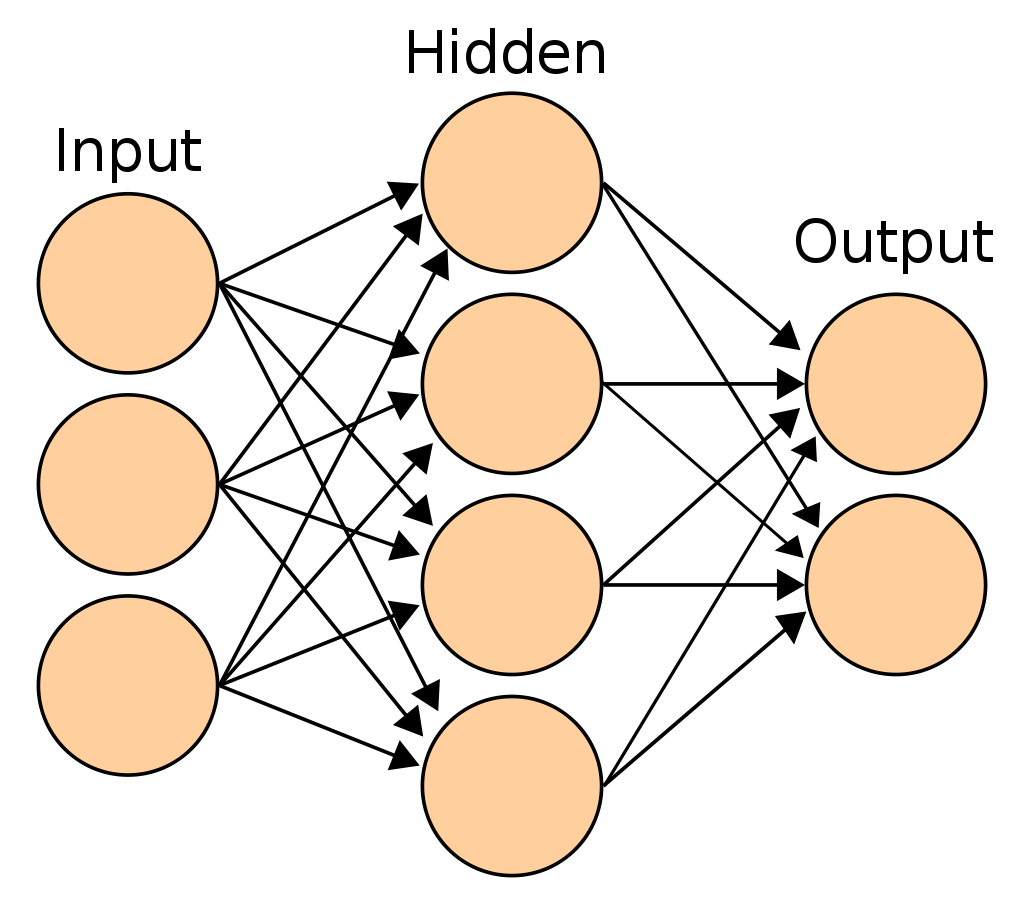
\includegraphics[height=0.4\textheight]{nn.png}
      \caption*{The expressivity and toolset of neural networks...}
    \end{subfigure}\pause
    \hspace{0.75cm}
    \begin{subfigure}[b]{.45\textwidth}
      \centering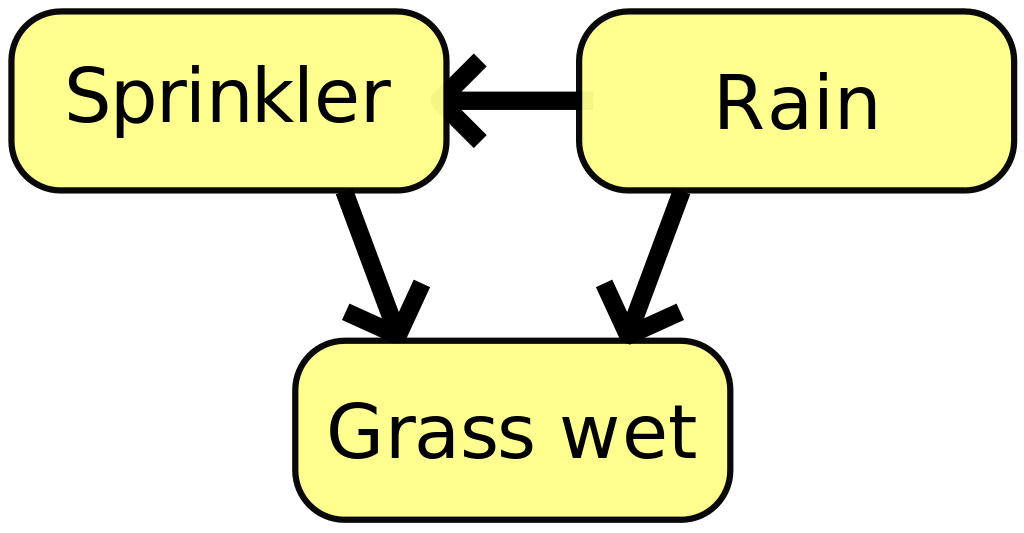
\includegraphics[height=0.3\textheight]{bnet.png}
      \vspace{0.25cm}
      \caption*{... and the interpretability and probabilistic semantics of PGMs.}
    \end{subfigure}
  \end{figure}
\end{frame}

\begin{frame}
  \frametitle{Sum-Product Network (SPN)}

  Sum-product networks (SPNs) are density estimators with a deep architecture.

  \begin{figure}
    \centering
    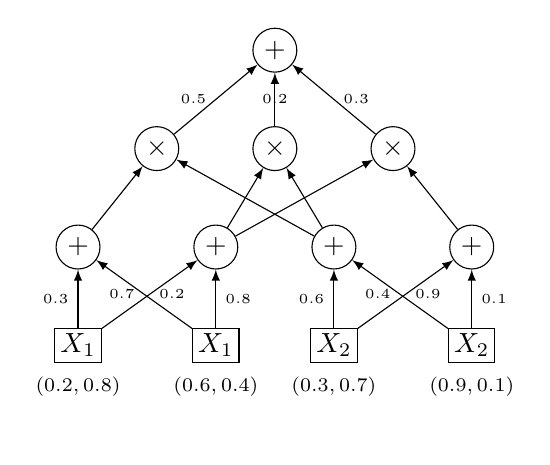
\begin{tikzpicture}
      \begin{scope}[every node/.style={circle,draw,inner sep=2pt}]
        \node (root) at (0, 0) {$+$};
        \node (p1) at (-1.5, -1.25) {$\times$};
        \node (p2) at (0, -1.25) {$\times$};
        \node (p3) at (1.5, -1.25) {$\times$};
        \node (s1) at (-2.5, -2.5) {$+$};
        \node (s2) at (-0.75, -2.5) {$+$};
        \node (s3) at (0.75, -2.5) {$+$};
        \node (s4) at (2.5, -2.5) {$+$};
        \node[draw,fill=none,rectangle,label={[label distance=-10pt]below:\scriptsize$(0.2, 0.8)$}] (x11) at (-2.5, -3.75) {${X}_1$};
        \node[draw,fill=none,rectangle,label={[label distance=-10pt]below:\scriptsize$(0.6, 0.4)$}] (x12) at (-0.75, -3.75) {${X}_1$};
        \node[draw,fill=none,rectangle,label={[label distance=-10pt]below:\scriptsize$(0.3, 0.7)$}] (x21) at (0.75, -3.75) {${X}_2$};
        \node[draw,fill=none,rectangle,label={[label distance=-10pt]below:\scriptsize$(0.9, 0.1)$}] (x22) at (2.5, -3.75) {${X}_2$};
      \end{scope}
      \begin{scope}[every path/.style={->},>=latex]
        \draw (p1) -- node[left]{\tiny$0.5$} (root);
        \draw (p2) -- node{\tiny$0.2$} (root);
        \draw (p3) -- node[right]{\tiny$0.3$} (root);
        \draw (s1) -- (p1);
        \draw (s3) -- (p1);
        \draw (s2) -- (p2);
        \draw (s3) -- (p2);
        \draw (s2) -- (p3);
        \draw (s4) -- (p3);
        \draw (x11) -- node[left]{\tiny$0.3$} (s1);
        \draw (x12) -- node[left]{\tiny$0.7$} (s1);
        \draw (x11) -- node[right]{\tiny$0.2$} (s2);
        \draw (x12) -- node[right]{\tiny$0.8$} (s2);
        \draw (x21) -- node[left]{\tiny$0.6$} (s3);
        \draw (x22) -- node[left]{\tiny$0.4$} (s3);
        \draw (x21) -- node[right]{\tiny$0.9$} (s4);
        \draw (x22) -- node[right]{\tiny$0.1$} (s4);
      \end{scope}
    \end{tikzpicture}
  \end{figure}
\end{frame}

\section{Learning SPNs}

\begin{frame}
  \frametitle{Learning SPNs}

  \begin{description}
    \item[Structure]
      \begin{itemize}
        \item Poon dense architecture\nocite{poon-domingos}
        \item LearnSPN\nocite{gens-domingos}
        \item Clustering architecture\nocite{clustering}
        \item Random-Tensorized SPNs\nocite{deep-learn-spn}
        \item ID-SPNs\nocite{id-spn}
        \item SPNs + Chow-Liu Trees\nocite{vergari-mauro}
      \end{itemize}
    \item[Parameter]
      \begin{itemize}
        \item Gradient descent;\nocite{poon-domingos,diff-approach-darwiche}
        \item Expectation-Maximization;\nocite{discriminative}
        \item Extended Baum-Welch;\nocite{baum-welch}
        \item Collapsed Variational Inference;\nocite{variational-spn}
        \item Concave-convex procedure;\nocite{cccp}
        \item Bayesian Moment Matching.\nocite{bayesian-moment}
      \end{itemize}
  \end{description}
\end{frame}

\section{Results}

\begin{frame}
  \frametitle{Some results}

  Not quite there yet on the discriminative side...

  \begin{table}
    \caption*{MNIST classification accuracy results}
    \begin{tabular}{l|l|l|l}
      LearnSPN & ID-SPN & SPN-SVD & DSPN-SVD\\
      \hline
      \vspace{0.5cm}
      81.8\% & 84.4\% & 85\% & 97.6\%\\
      SPN-TH & RAT-SPN & Prometheus & DC-SPN\\
      \hline
      98.34\% & 98.19\% & 98.37\% & 99.19\%
    \end{tabular}
  \end{table}
  \vspace{0.5cm}

  ...but gradually getting better.
\end{frame}

\begin{frame}
  \frametitle{More results}

  SPNs shine on generative tasks!

  \begin{figure}
    \begin{subfigure}{0.49\textwidth}
      \centering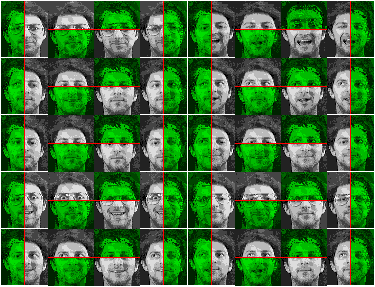
\includegraphics[width=\textwidth]{cmpl_0.png}
    \end{subfigure}
    \begin{subfigure}{0.49\textwidth}
      \centering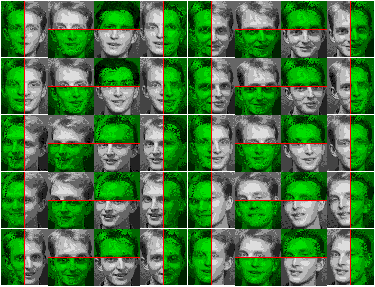
\includegraphics[width=\textwidth]{cmpl_1.png}
    \end{subfigure}
    \caption{Image reconstruction}
  \end{figure}
\end{frame}

\section{Applications}

\begin{frame}
  \frametitle{Applications}

  SPNs have reached incredible results in different fields:
  \vspace{0.5cm}

  \begin{itemize}
    \item Image segmentation, classification and completion
    \item Protein folding
    \item Speech recognition
    \item Natural language processing
    \item Semantic mapping and control in robotics
    \item Activity recognition
    \item Semantic Web
  \end{itemize}
\end{frame}

\begin{frame}
  \begin{center}
    \huge Thank you!
  \end{center}
\end{frame}

\begin{frame}[t,allowframebreaks]
  \frametitle{References}
  \printbibliography[heading=none]
\end{frame}

\end{document}
